\chapter{Untersuchung der Messdaten}
Um eine Aussage über die Qualität des Touchscreen treffen zu können, werden mehrere Untersuchungen angestellt. 

Bei der ersten Untersuchung wird auf die Mitte des Touchscreen gedrück und die Position wird für eine gewisse Zeit gehalten.
Die Daten werden anschließen ausgewertet (siehe Abschnitt \ref{ab:genau}).

Um die erste Untersuchung zu erweitern wird nun die Mitte des Touchscreen wiederholt gedrückt. Hier bei soll die Wiederholbarkeit eines Punktes auf dem Touchscreen untersucht werden. 
Die Auswertung ist in Abschnitt \ref{ab:wiederholung} zu finden.

Bei der letzen Untersuchung wird die Linearität des Touchscreen untersucht. Hierfür gibt der Hersteller eine Garantie, unter der sich die Linearität des Touchscreen befinden soll. 
Den Wert der angegeben wird liegt bei \SI{1,5}{\%} (siehe \ref{ds:touch} Seite 3 des Datenblatts).

Um die Nachfolgende Untersuchungen korrekt durchführen zu können muss zu nächst der Reaktionsbereich des Touchscreens ermittelt werden.
Durch seine Bauform hat dies einen Randbereich an dem es nicht zu verlässig Werte ausgibt. Umkehrschluss, das Programm erkennt nicht das etwas den Touchscreen betätigt. 
Im Datenblatt werden Werte für den Bereich genannt in dem es zuverlässig arbeitet. In X-Richtung hat der Touchscreen einen Arbeitsbereich von \SI{212,2}{mm} und in Y-Richtung eine Bereich von \SI{159,4}{mm} (siehe Datenblatt \ref{ds:touch}).

Durch Ausprobieren wurden die maximal und minimal ADC-Werte in die jeweilige Richtung ermittelt. Mit Hilfe dieser Werte ist es möglich die jeweiligen ADC-Werte in das metrische System zuüberführen.
\begin{table}[ht!]
    \caption{maximal und minimal ADC-Werte}
    \begin{center}
        \begin{tabular}{ c |c| c }
            
                & x-Richtung & y-Richtung \\ \hline
         max. ADC-Werte & 954 & 913 \\  \hline
         min. ADC-Werte& 69 & 102 \\   
        \end{tabular}
    \end{center}   
\end{table}

Mit diesen Werten lassen sich der jeweilige Gesamt-Offset in jede Richtung bestimmen.
\begin{align}
    ADC_{x,offset} &= 69 +(1024-954)\nonumber\\
    ADC_{x,offset} &= 139\label{eq:adcxoffset}\\
    ADC_{y,offset} &= 102+(1024-913)\nonumber\\
    ADC_{y,offset} &= 213\label{eq:adcyoffset}
\end{align}

\section{Genauigkeit bei konstanten Koordinaten}
\label{ab:genau}
\begin{figure}[ht!]
    \centering
    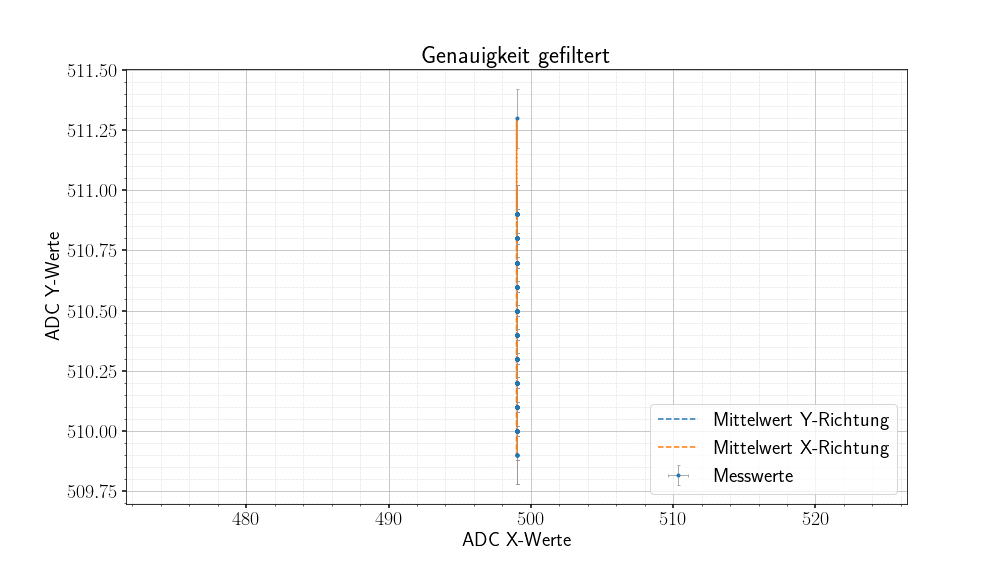
\includegraphics[width=\linewidth]{fig/filtered.png}
    \caption{}
    \label{fig:filtered}
    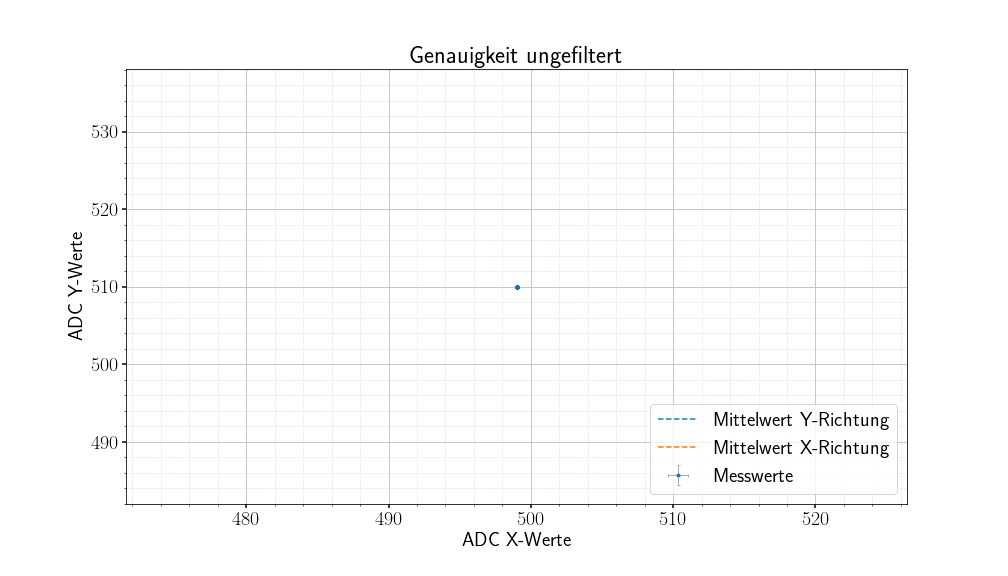
\includegraphics[width=\linewidth]{fig/unfiltered.png}
    \caption{}
    \label{fig:unfiltered}
\end{figure}
\section{Reproduzierbarkeit von Koordinaten}
\label{ab:wiederholung}
\begin{figure}[ht!]
    \centering
    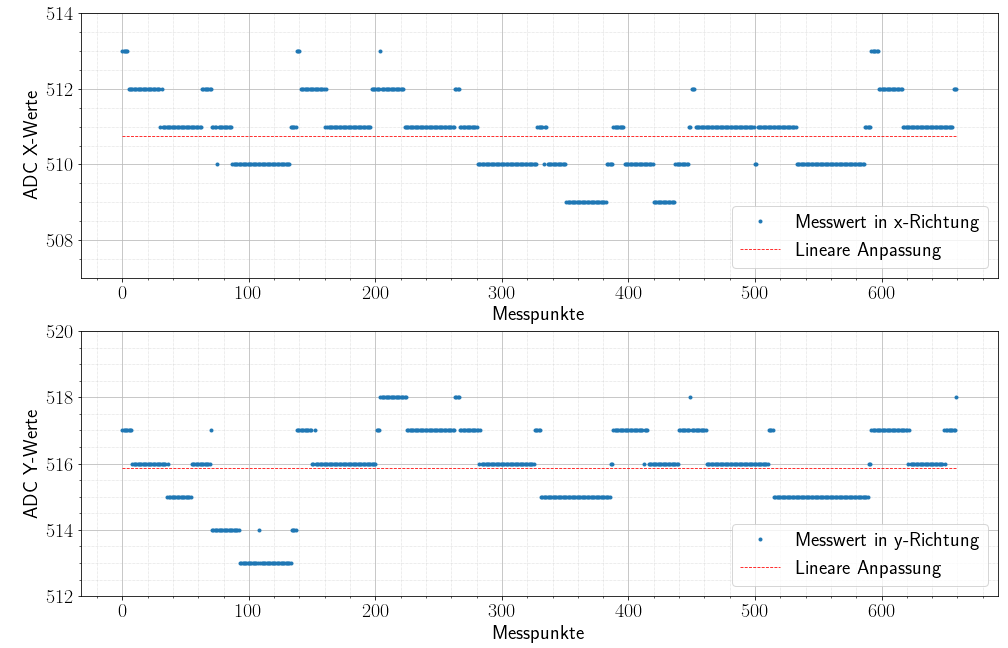
\includegraphics[width=\linewidth]{fig/wiederholung.png}
    \caption{}
    \label{fig:wiederhol}
\end{figure}
\section{Linearität in x- und y-Richtung}
\label{ab:linear}
\begin{figure}[ht!]
    \centering
    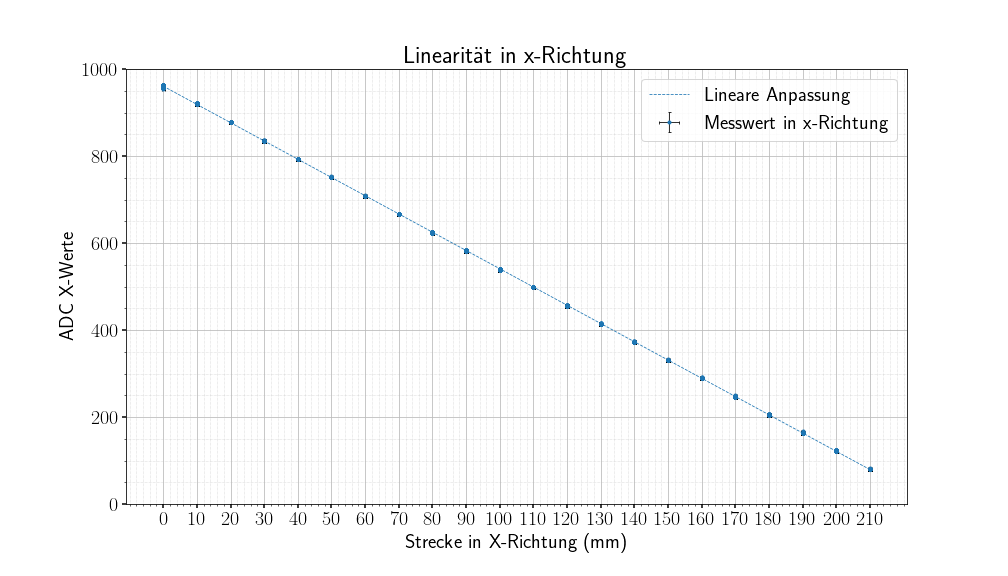
\includegraphics[width=\linewidth]{fig/8_linearitaet_x.png}
    \caption{}
    \label{fig:xlinear}
    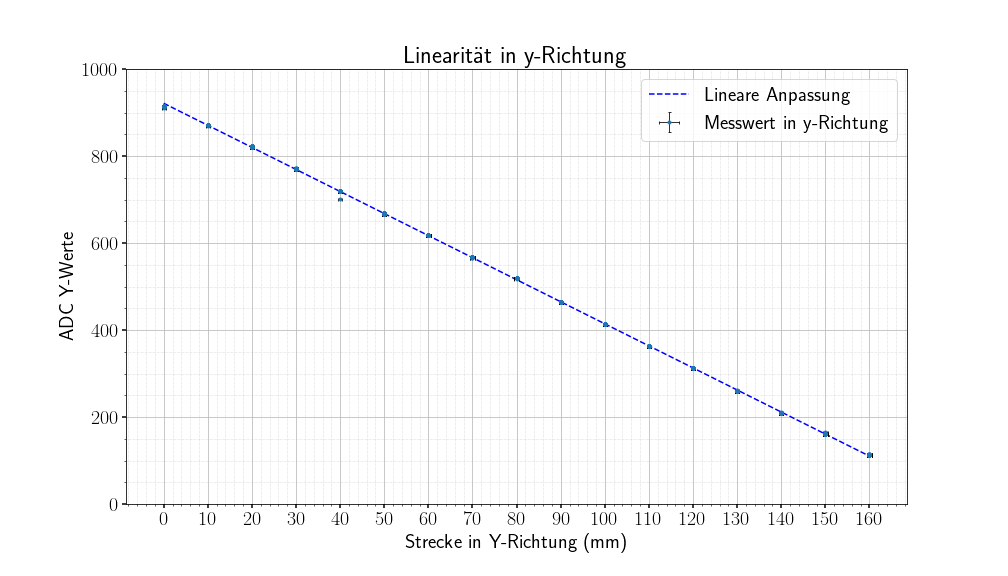
\includegraphics[width=\linewidth]{fig/8_linearitaet_y.png}
    \caption{}
    \label{fig:ylinear}
\end{figure}